\documentclass[a4paper,14pt]{extarticle} 
\usepackage[a4paper,top=1.5cm, bottom=1.5cm, left=2cm, right=1cm]{geometry}
%\usepackage[T2A]{fontenc}
%\usepackage[english, russian]{babel}
\usepackage{graphicx}
\DeclareGraphicsExtensions{.pdf,.png,.jpg}
\usepackage{fontspec}
\setmainfont{Times New Roman}
\setsansfont{FreeSans}
\setmonofont{FreeMono}
\renewcommand{\baselinestretch}{1.5}
\usepackage{polyglossia}
\setdefaultlanguage{russian}
\setotherlanguages{english,russian}
\usepackage{setspace}
\usepackage[many]{tcolorbox}
\usepackage{listings}
\usepackage{multicol}
\usepackage{xcolor}
\usepackage{pdfpages}

\definecolor{codegreen}{rgb}{0,0.6,0}
\definecolor{codegray}{rgb}{0.5,0.5,0.5}
\definecolor{codepurple}{rgb}{0.58,0,0.82}
\definecolor{backcolour}{rgb}{0.95,0.95,0.92}

\lstdefinestyle{mystyle}{
    backgroundcolor=\color{backcolour},   
    keywordstyle=\color{magenta},
    numberstyle=\tiny\color{codegray},
    stringstyle=\color{codepurple},
    basicstyle=\ttfamily\footnotesize,
    breakatwhitespace=false,         
    breaklines=true,                 
    captionpos=b,                    
    keepspaces=true,                 
    numbers=left,                    
    numbersep=5pt,                  
    showspaces=false,                
    showstringspaces=false,
    showtabs=false,                  
    tabsize=2
}

\lstset{style=mystyle}

\begin{document}
    \begin{center}
        \thispagestyle{empty}
        \begin{singlespace}
        ФЕДЕРАЛЬНОЕ АГЕНТСТВО СВЯЗИ

        ФЕДЕРАЛЬНОЕ ГОСУДАРСТВЕННОЕ БЮДЖЕТНОЕ ОБРАЗОВАТЕЛЬНОЕ

        УЧРЕЖДЕНИЕ ВЫСШЕГО ОБРАЗОВАНИЯ

        «САНКТ-ПЕТЕРБУРГСКИЙ ГОСУДАРСТВЕННЫЙ УНИВЕРСИТЕТ ТЕЛЕКОММУНИКАЦИЙ ИМ. ПРОФ. М.А. БОНЧ-БРУЕВИЧА»

        (СПбГУТ)
        \end{singlespace}
        \vspace{-1ex}
        \rule{\textwidth}{0.4pt}
        \vspace{-5ex}

        Факультет \underline{Инфокоммуникационных сетей и систем}

        Кафедра \underline{Защищенных систем связи}
        \vspace{10ex}

        \textbf{Лабораторная работа №2}\\
        Авторизация сетевых соединений
        


    \end{center}
    \vspace{4ex}
    \begin{flushright}
    \parbox{10 cm}{
    \begin{flushleft}
        Выполнили студенты группы ИКТЗ-83:

        \underline{Громов А.А., Миколаени М.С., Мазеин Д.С.} \hfill 

        \footnotesize \textit{ (Ф.И.О., № группы)} \hfill \rule[-0.85ex]{0.1\textwidth}{0.6pt}
        
        \hfill \textit{(подпись)} \normalsize

        Проверил:

        \underline{Казанцев А.А.} \hfill \rule[-0.85ex]{0.1\textwidth}{0.6pt}

        (\footnotesize \textit{уч. степень, уч. звание, Ф.И.О.) \hfill (подпись)} \normalsize

    \end{flushleft}
    }
    \end{flushright}
    \begin{center}
        \vfill
        Санкт-Петербург

        2021

    \end{center}
    \newpage


    \textbf{Пункт 2}
    \vspace{-3ex}
    \begin{center}
        \singlespacing
        В данном пункте мы убедились, что передается открытый трафик с помощью программы Wireshark.

        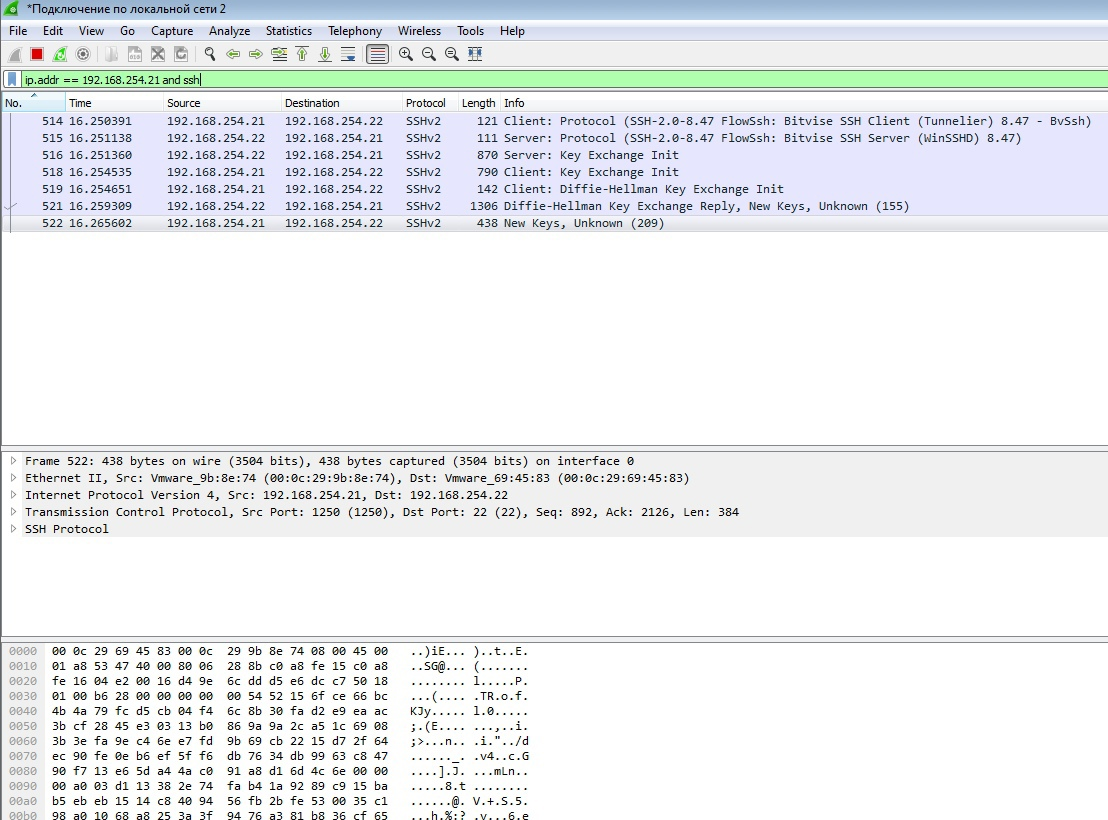
\includegraphics[scale=0.3]{pics/2.jpg}

       Рис. 1 Открытый трафик. 
    \end{center}

    \textbf{Пункт 3}
    \vspace{-3ex}
    \begin{center}
        \singlespacing
        В данном пункте мы настроили правила доступа, разрешающее всем сетевым сервисам входящее подкючение. 

        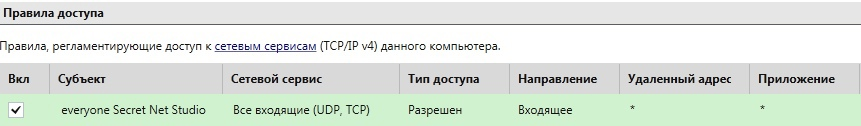
\includegraphics[scale=0.5]{pics/3.jpg}

        Рис. 2 Парвило доступа.
    \end{center}

    \textbf{Пункт 4}
    \vspace{-3ex}
    \begin{center}
        \singlespacing
        В данном пункте мы настроили режим защиты сетевых соединений.

        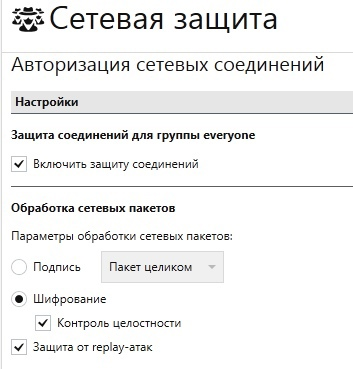
\includegraphics[scale=0.6]{pics/4.jpg}

        Рис. 3 Экран настрокий.
    \end{center}

    \textbf{Пункт 5}
    \vspace{-3ex}
    \begin{center}
        \singlespacing
        В данном пункте мы увидели, что трафик не зашифровался.

        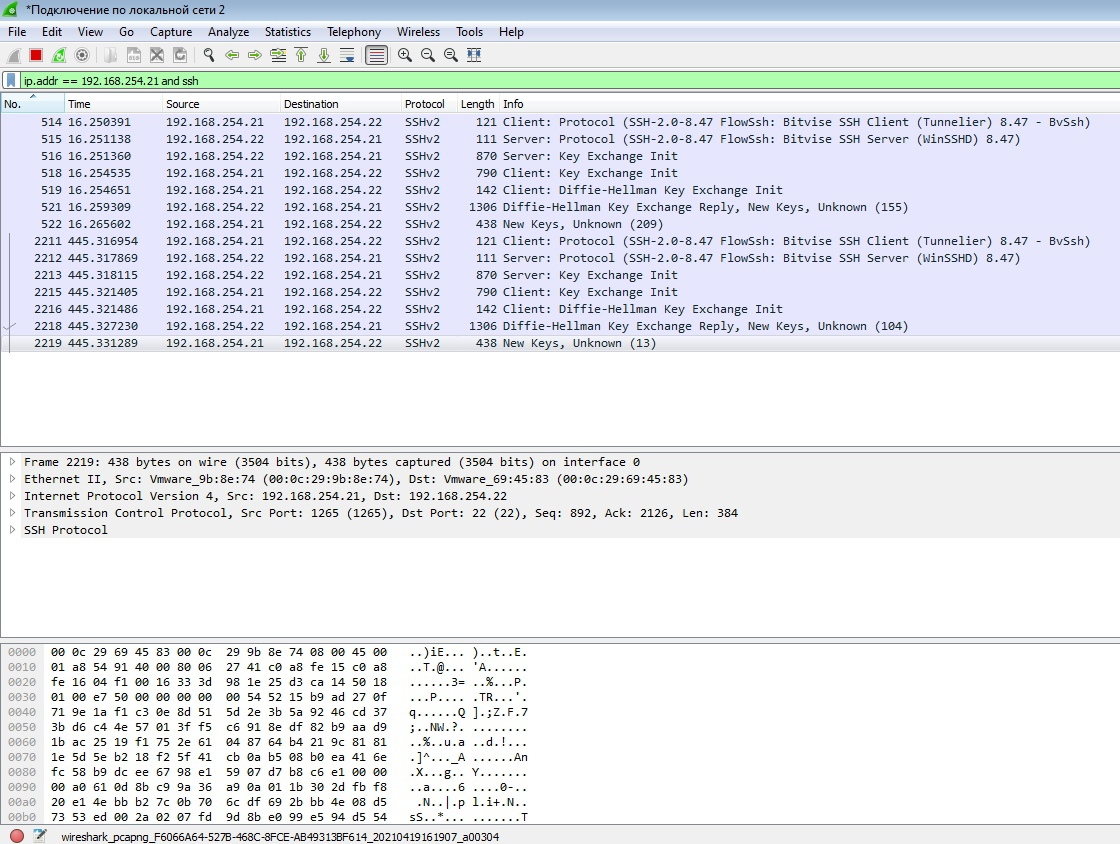
\includegraphics[scale=0.3]{pics/5.jpg}

        Рис. 4 Не удалось защифровать трафик.
    \end{center}

    \textbf{Пункт 7}
    \vspace{-3ex}
    \begin{center}
        \singlespacing
        В данном пункте мы настроили блокировку соединений для неавторизованных на СБ пользователей

        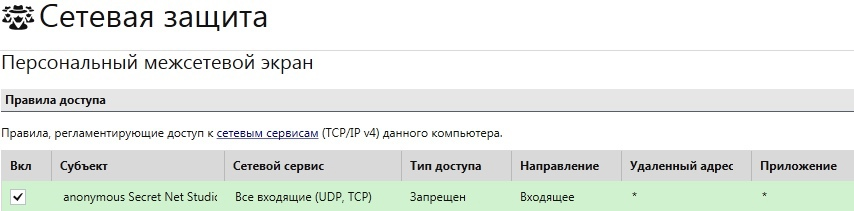
\includegraphics[scale=0.5]{pics/7.jpg}

        Рис. 5 Парвило доступа.
    \end{center}

    \textbf{Вывод}\par
    Выполнив данную лабораторную работу, мы протестировали компонент "Авторизация сетевых соединений" в Secret Net Studio. 

    \newpage
    \textbf{Ответы на контрольные вопросы.}
    \begin{enumerate}
        \singlespacing
        \item \textbf{В чем заключается особенность функционирования ПМЭ в Secret Net \linebreak Studio,
        отличающая его от традиционных, "периметровых" МЭ?}\par
        В отличие от традиционных, "периметровых" МЭ, реализованный в SNS \linebreak
        распределенный межсетевой экран предназначен именно для защиты \linebreak информации 
        внутри сети организации, функционирует непосредственно на ее защищаемых объектах 
        (сервер БД, рабочие места руководителей или сотрудников и т.д.) и обеспечивает 
        их защиту от сетевых угроз со стороны внешнего и внутреннего нарушителей.
        \item \textbf{Какие группы правил проверки сетевого трафика реализованы в ПМЭ Secret
        Net Studio?}\par
        Правила доступа, прикладные правила, системные правила, сетевые протоколы.
        \item \textbf{Какая из групп правил проверки сетевого трафика в ПМЭ Secret Net Studio
        имеет наивысший приоритет? Что регламентируется правилами этой \linebreak группы?}\par
        Системные правила. Регламентируют доступ к защищаемым ПК по сетевым протоколам.
        \item \textbf{По каким протоколам может ограничиваться доступ к защищаемым \linebreak ресурсам
        с помощью системных правил?}\par
        Все IP-based протоколы (Например RDP)
        \item \textbf{Какая из групп правил проверки сетевого трафика в ПМЭ Secret Net Studio
        имеет минимальный приоритет? Что регламентируется правилами этой
        группы?}\par
        Прикладные правила. Регламентируют доступ пользователей к сетевым сервисам защищаемого компьютера (например, общие папки).
        \item \textbf{Каков порядок обработки заданных в параметрах ПМЭ Secret Net Studio
        правил доступа?}\par
        Чем выше правило в таблице, тем больше его приоритет
        \item \textbf{Через какой промежуток времени после сохранения изменений вступают в
        силу новые настройки правил доступа ПМЭ Secret Net Studio?}\par
        4 - 6 минут
        \item \textbf{Какой режим работы ПМЭ в Secret Net Studio позволяет составить на основе
        информации о сетевой активности приложений базовый набор \linebreak правил
        доступа, необходимый для функционирования защищаемого \linebreak компьютера?}\par
        Сетевой режим
        \item \textbf{В чем заключается особенность аутентификации пользователей механизмом
        авторизации сетевых соединений Secret Net Studio?}\par
        Механизм авторизации сетевых соединений обеспечивает защиту \linebreak взаимодействия только между авторизованными на СБ клиентами Secret Net Studio. Если на компьютере пользователя не установлен Secret Net Studio или пользователь по каким-либо причинам не прошел аутентификацию на СБ SNS (anonymous), то трафик между ним и авторизованным клиентом SNS не будет защищаться.
        \item \textbf{Какими средствами обеспечивается защита и целостность передаваемых
        данных в механизме авторизации сетевых соединений?}\par
        Средствами протоколов семейства IPsec, а именно AH (Authentication Header) - гарантирует аутентичность и целостность и ESP (Encapsulation Security Payload) - шифрование и контроль целостности.
        \item \textbf{Что необходимо для возможности выбора пользователя или группы \linebreak
        пользователей, доступ к которой будет контролироваться при создании
        нового правила доступа в параметрах настроек политик ПМЭ?}\par
        Необходима лицензия на использование механизма авторизации сетевых \linebreak соединений.
        \item \textbf{Наличие каких правил необходимо для работы прикладных правил доступа
        к общим папкам на защищаемом компьютере?}\par
        Если прохождение пакетов по протоколу SMB запрещается системными \linebreak правилами
        или правилами доступа, то прикладные правила не работают, так как на транспортном уровне IP-пакеты блокируются.
    \end{enumerate}
\end{document}

